\documentclass[tikz]{standalone}

%!TEX root = main.tex

% mytikzset
\usepackage{tikz}
\usetikzlibrary{positioning,arrows,shapes,patterns}
\usetikzlibrary{decorations.pathmorphing}
\usetikzlibrary{decorations.markings}
\usetikzlibrary{decorations.pathreplacing}
\usetikzlibrary{calc}
\usetikzlibrary{patterns}
\usetikzlibrary{decorations.markings}
\usetikzlibrary{petri}

\tikzset{
  vector/.style={thick,double,draw=black, postaction={decorate},
    decoration={markings,mark=at position .6 with {\arrow[black,scale=0.4]{triangle 45}}}},
  axial/.style={thick,double,densely dashed,draw=black, postaction={decorate},
    decoration={markings,mark=at position .6 with {\arrow[black,scale=0.4]{triangle 45}}}},
  gluon/.style={decorate, draw=black,
    decoration={coil,aspect=0.3,segment length=5pt,amplitude=3pt}},
  pseudo/.style={thick, dashed, draw=black, postaction={decorate},
    decoration={markings,mark=at position .6 with {\arrow[red,scale=0.5]{triangle 45}}}},
  scalar/.style={thick,draw=black, postaction={decorate},
    decoration={markings,mark=at position .6 with {\arrow[black,scale=0.5]{triangle 45}}}},
  cut/.style={draw=black, decorate, decoration={snake, segment length=1mm, amplitude=0.2mm}}
}


\usepackage{amsfonts}
\newcommand{\Po}{\ensuremath{\mathbb{P}}}

\begin{document}
\nopagecolor
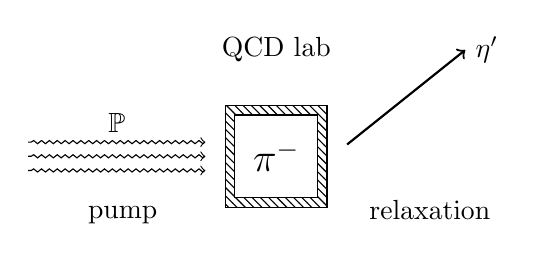
\begin{tikzpicture}[x=1.5cm, y = 1.5cm]
  \draw[] (-0.43,-0.43) rectangle (0.43,0.43);
  \fill[gray, pattern=north west lines] (-0.43,-0.43) rectangle (0.43,0.43);
  \draw[fill=white] (-0.35,-0.35) rectangle node[] {\Large$\pi^-$} (0.35,0.35);
  %%
  \draw[cut,<-] (-0.6,0.12) -- node[above] {\Po} ++(-1.5,0);
  \draw[cut,<-] (-0.6,0) --                      ++(-1.5,0);
  \draw[cut,<-] (-0.6,-0.12) --                  ++(-1.5,0);
  %%
  \draw[thick,->] (0.6,0.1) -- ++(1,0.8) node[right] {$\eta^{\prime}$};
  %%
  \node[] at (-1.3,-0.5) {pump};
  \node[] at ( 1.3,-0.45) {relaxation};
  \node[] at (0,0.9) {QCD lab};
\end{tikzpicture}
\end{document}
